\subsection{Segmentation}

The main objective of this project was to determine if the physicians/clinicians/technicians are able to obtain more meaningful information when given more depth information through a holographic print.  To give this type of information, structural patterns within the model must be apparent. To achieve this we used a data-set of a human brain containing a tumor. We believe that the depth information inherently found in holography, will make the location of the tumor become apparent.  As an intermediate step we need to develop geometry for each of the salient structures of the brain, mainly the white and gray matter, as well as the tumor and other abnormal tissues surrounding the tumor.  This is where segmentation algorithms are needed.\\

There are several different approaches that have been found throughout the literature \cite{pham2000current}.  But they all stem from the same set of core ideas.  In this project we explored both automatic and semi-automatic methods.

\subsubsection{Automatic}

One of our ultimate goal of the project is to use existing software and have a file-print process in which the MRI data is generated directly into a holographic print without any human intervention.  This automatic approach from MRI to holographic print needs automatic annotation and segmentation of the MRI data.  Current methods include the annotation and segmentation of each of the slices. This is inefficient and also time consuming. In this section we will explore the possibility of automating this step using transfer leaning and 3D U-Net dense volumetric segmentation\cite{cciccek20163d}.\\

One of the main issues using deep learning methods in the medical field, is the lack of a large enough sample size for the network to fully stabilize the weights and biases.  To overcome this issue it is often the case that we have to use transfer learning techniques using pre-trained networks.  In this project we explored the possibility of using inductive transfer learning\cite{pan2010survey} and a pre-trained network found in the work of \cite{cciccek20163d}.  Using transfer learning, instead of starting the learning process from the beginning, the learning process starts from patterns that have been learned when solving a different or similar problem. In this way, we essentially utilize previous learning's from the pre-trained network and apply them to our dataset.\\

The work done by \cite{cciccek20163d} expands the work previously achieved by \cite{ronneberger2015u} but using 3D volumetric data.  There is an added dimension of depth in all filters and weights in the U-Net architecture.  The depth information comes from the slice information in the MRI. During the encoder or down sampling portion of the architecture two 3 x 3 x 3 convolutions were performed followed by a rectified linear unit (ReLu).  This was followed up by a single 2 x 2 x 2 max pooling with strides of 2 in each dimension.  In the synthesis or up-convolution path a 2 x 2 x 2 with strides of 2 in each dimension was used followed by the mirrored 3 x 3 x 3 convolution with ReLu.  To reduce bottle-necking doubling the channels was done before each max pooling layer.  In the last layer a 1 x 1 x 1 x 1 convolution was used for the output layer for each of the labeled cases white matter, gray matter, tumor and abnormal tissue. The last layer used a weighted softmax loss function.  Note that the input layer was 256 x 256 x 118.

\begin{figure}[H]
  \centering
  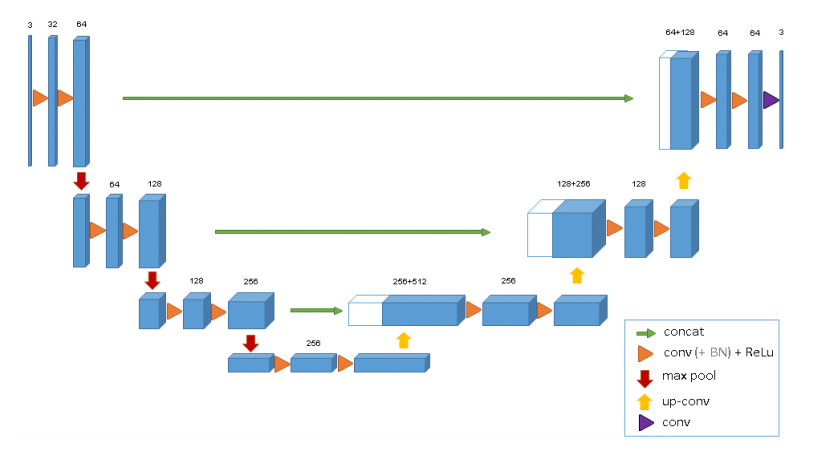
\includegraphics[width=\linewidth]{img/volumetricUNetArchitecture.PNG}
  \caption{UNet architecture used in Cicek et.el. \cite{cciccek20163d}}
  \label{fig:uNet}
\end{figure}

In theory this approach would have worked but the data used by \cite{cciccek20163d} was too different from the data we are using, so the transfer learning did not give us the adequate segmentation we wanted.  Due to the limited time of the project this was abandoned and semi-automatic techniques were more focused as they are more intuitive and don't require a large sample size.  In the future we would like to pursue this approach as this would be more akin to our ultimate goal of the file-print process.


\subsubsection{Semi-Automatic}

Since the brain consists of known tissue types such as white and gray matter, bone and spinal fluid, the intuitive approach would be to classify these based on intensity values of the pixels on the MRI \cite{atkins1998fully}.  The problem arises when there are overlapping tissues in which case the intensity values of each pixel will be miss classified as one of the known tissue types \cite{undeman2003fully}.  This is why current MRI segmentation is not fully automated and radiologists are needed to help the computer identify which pixels are wrong and correct it. To combat this issue, there are some algorithms such as the one proposed by \cite{lenroot2006brain} whereby they use pre-segmented brain template and perform image registration and automatically identify the troublesome pixels and fix the labels accordingly.\\  

However necessary, the main purpose of this project is not on segmentation rather exploring the depth information of the digital holographic print.  So we will not use complex segmentation techniques, instead we will use the more intuitive approach of pixel classification using multithresholding (MT) techniques \cite{sahoo1988survey} in combination with region growing approaches\cite{adams1994seeded}.\\

The overall goal of MT is to generate masks which partition the image into our desired segmented areas.  To do this a histogram is first generated to identify the threshold ranges of each tissue type.  The segmentation is achieved by grouping similar pixel intensities together akin to quantizing the image.  But in this case the quantization levels are not constant. This is clearly seen in figure \ref{fig:mriHistogram}.  In the MRI you can see three distinct colours which corresponds to the white and gray matter (WM,GM) and also the cerebral fluid (CSF).  The histogram distributions show 3 distinct peak which corresponds to these tissue types.

\begin{figure}[H]
  \centering
  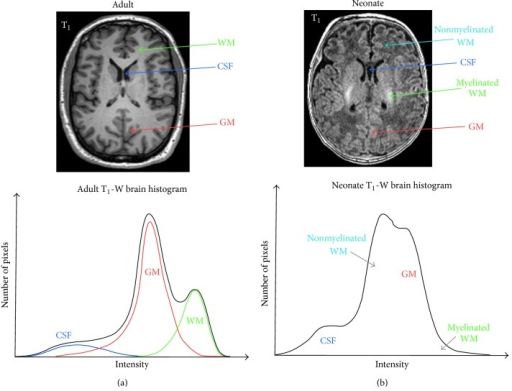
\includegraphics[width=\linewidth]{img/mriHistogram.png}
  \caption{MRI and pixel intensity histogram distribution.}
  \label{fig:mriHistogram}
\end{figure}

Notice the problem described earlier, there are overlapping pixels in the histogram that can be in either of the 3 labeled tissue classes.  We will combat this problem by introducing a region growing approach.\\

Region growing is a simple yet effective technique which samples and extracts a region of the image by connecting similar pixels together. Though very similar to thresholding, this introduces a fuzzy thresholding approach rather than categorical quantization.  The fuzzy approach comes about through the corporation of both the intenisty and edges of the image. The main step is to add a seed point which is manually selected, and from this point connect all the pixels surrounding it together and label that region accordingly.  In the literature this is often done for tumor and lesion segmentation\cite{guliato1998segmentation}. The main disadvantage of this approach is the resultant mask can be very noisy causing the extracted region to have holes and disconnected regions.  To remedy this affect we applied morphological filters\cite{mendiola2007morphological}.\\

Our python implementation can be found in Appendix \ref{sec:appendixPythonFunction}.